\usetikzlibrary{arrows,positioning}
\tikzset{%
 % >={Latex[width=2mm,length=2mm]},
  % Specifications for style of nodes:
            base/.style = {circle,draw=black, minimum width=1cm,minimum height=1cm,
                           text centered, font=\Large\sffamily},
  tensorflow/.style = {base, fill=blue!30},
       tati/.style = {base, fill=red!30},
       tati_highlevel/.style = {base, fill=green!60},
     pydiffmap/.style = {base, fill=blue!60},
%          process/.style = {base, minimum width=2.5cm, fill=orange!15,
%                            font=\ttfamily},
pil/.style={
           ->,
           very thick,
           shorten <=3pt,
           shorten >=3pt,}
}

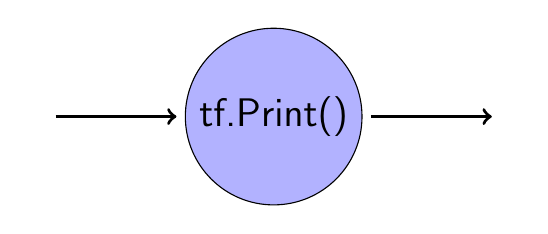
\begin{tikzpicture}[node distance=3cm,
    every node/.style={fill=white, font=\sffamily}, align=center]

\node (a)	[draw=white]	{};
\node (b)	[tensorflow,right of=a]	{tf.Print()};
\node (c)	[draw=white,right of=b]	{};

\draw[pil] (a) -- (b);
\draw[pil] (b) -- (c);

\end{tikzpicture}